%*******************porque no veo que esté*************************************************************************
%								COMANDOS ÚTILES PARA LATEX EN ESTE TP							
%
%	\ : espacio simple
%	\\ : nueva l\'inea
%	\par : va a la l\'inea de abajo y deja sangr\'ia
%	\vspace{##tamaño en pt##} o \vspace{\baselineskip} en general:
%								 para dejar un espacio vertical
%	\textbf{text} :text en negrita
%	\textit{text} :text en itálica
%
% GRAFICOS CENTRADOS:
%	\begin{center}
%		\includegraphics[width=\textwidth]{./img/##ruta imagen (no hace falta extension)##}
%	\end{center}
%		--> se pueden agregar atributos como scale por si se hace muy grande
%
% TABLAS CENTRADAS:
%	\begin{center}
%	\begin{tabular}{|c|c|}
%	\hline
%	\ \textbf{Programa} & \textbf{Ticks} \\
%	\hline
%		ASM & 675127609 \\
%	\hline
%	\end{tabular}
%	\end{center}
%
% ALGORITMOS (EN VARIOS LENGUAJES):
% \begin{lstlisting}
%	void sumoDiez(int &num)
%	{
%	    num += 10;
%	}
%	
%	int main()
%	{
% 	   int i;
%	    int numeroAProcesar = 20;
%	    for (i = 0; i < 50; i++)
%	    {
%	        sumoDiez(numeroAProcesar);	//Proceso el numero en cada ciclo
%	    } 
%	    return 0;
%	}
%	\end{lstlisting}
%
% para info sobre todo lo que tiene el package detallado:
% http://en.wikibooks.org/wiki/LaTeX/Source\_Code\_Listings
%
%********************************************************************************************

\documentclass[10pt,a4paper]{article}
\usepackage[utf8]{inputenc} % para poder usar tildes en archivos UTF-8
\usepackage[spanish]{babel} % para que comandos como \today den el resultado en castellano
\usepackage{a4wide} % márgenes un poco más anchos que lo usual
\usepackage[conEntregas]{caratula}
\usepackage{amssymb}
\usepackage{fancybox}
\usepackage[usenames,dvipsnames]{color}
\usepackage{hyperref}
\usepackage{listings}
\usepackage{xcolor}
\usepackage{amsmath}
\usepackage{pdflscape}
\usepackage{listings}

\hypersetup{
    colorlinks,
    citecolor=black,
    filecolor=black,
    linkcolor=black,
    urlcolor=black
}

\lstdefinestyle{customc}{
  belowcaptionskip=1\baselineskip,
  breaklines=true,
  frame=L,
  xleftmargin=\parindent,
  language=C,
  showstringspaces=false,
  basicstyle=\footnotesize\ttfamily,
  keywordstyle=\bfseries\color{green!40!black},
  commentstyle=\itshape\color{purple!40!black},
  identifierstyle=\color{blue},
  stringstyle=\color{orange},
}

\lstset{escapechar=@,style=customc}

\begin{document}

\titulo{Trabajo Práctico 1}
\subtitulo{Análisis preliminar del sistema de software “TecnoTaxi”}

\fecha{\today}

\materia{Ingenier\'ia del Software I}
\grupo{}

\integrante{Barbeito, Nicolás}{147/10}{nicolasbarbeiton@gmail.com}
\integrante{Chapresto, Mat\'ias}{201/12}{matiaschapresto@gmail.com}
\integrante{Garassino, Agust\'in Javier}{394/12}{ajgarassino@gmail.com}
\integrante{Sarriés, Ana}{144/02}{anasarries@yahoo.com.ar}
\integrante{Vileriño, Silvio}{106/12}{svilerino@gmail.com}

\maketitle

\tableofcontents
\newpage

\section{Descripción general del sistema}
El objetivo del sistema es automatizar las solicitudes de taxis por parte de los pasajeros y la coordinación de los viajes con los taxistas. Para lograr esto se desarrollará una aplicación web, con la cual interactuarán tanto los clientes como los empleados de la empresa de RadioTaxi. Los pasajeros podrán comunicarse a través de internet para solicitar los viajes ya sea utilizando un dispositivo móvil o una computadora de escritorio. Tendrán la opción de elegir dentro de un listado de perfiles de choferes con información sobre: el modelo del auto, puntuación asignada según antiguos pasajeros, etc. A su vez los taxistas interactuarán con el sistema utilizando dispositivos móviles que serán prove\'idos por la empresa de RadioTaxi, ellos tendrán un listado de posibles viajes a realizar, pudiendo aceptar uno de ellos en cualquier momento. Además, con el fin de mejorar el servicio, información sobre la ubicación de los taxis será obtenida a través de un dispositivo de posicionamiento global GPS que se comunicará con el sistema a través de un servicio satelital prestado por terceros.

\subsection{Interacción con el pasajero}
La interacción de la plataforma con el pasajero será, como se mencionó anteriormente, a través de internet. Para tener acceso al sistema este deberá primero crear un usuario, indicando un mail y contraseña. Esto permitirá posteriormente obtener información estad\'istica de gran valor, además de permitir comunicarse con el pasajero en caso de que el viaje no pueda ser concretado por algún motivo. 

Un usuario puede solicitar un viaje a través de la aplicación web indicando el punto donde el taxi debe pasar a recogerlo, el destino y el horario. A esto la aplicación contestará con un listado de posibles taxistas elegidos convenientemente según las preferencias del usuario en base a información recopilada por el sistema, teniendo en cuenta también la ubicación actual de cada una de las unidades. El usuario puede proceder a seleccionar uno o varios de los taxistas, el sistema tendrá en cuenta la decisión del usuario pero el taxista al que se le asignará el viaje puede diferir.

Una vez determinado el taxista que se encargará del viaje el usuario será notificado. Finalmente el pasajero tendrá acceso a un menú de viajes pendientes en donde podrá visualizar la ubicación actual del taxi, además de tener la posibilidad de cancelar la solicitud. Una vez finalizado el viaje, el usuario puede puntuar al taxista positiva o negativamente. En caso de que el taxista cancele el viaje asignado, el usuario será notificado.

El pasajero podrá además utilizar la aplicación para reservar viajes periódicos seleccionando un taxista espec\'ifico entre los disponibles. En caso de que por algún motivo el taxista no pueda concurrir uno de los d\'ias especificados el usuario será informado. Estas reservas periódicas serán consideradas por el sistema a la hora de seleccionar los taxis libres para realizar viajes.

En caso de no disponer de acceso a internet, el pasajero podrá llamar a un operador humano con acceso al sistema. No es necesario que el pasajero disponga de una cuenta en la aplicación, el operador realizará toda la interacción con el sistema. Sin embargo, dado el inconveniente de la p\'erdida de conex\'ion, se pierde parte de la funcionalidad del sistema, como el acceso al listado de taxistas. El pasajero que se comunique por tel\'efono s\'olo podr\'a solicitar un taxi cualquiera, cancelarlo y solicitar el tiempo de espera.

\subsection{Interacción con el taxista}
Los perfiles de los taxistas serán cargados manualmente en la aplicación. Tendrán un taxi asociado y una puntuación determinada por los usuarios a través de un sistema de votación. Estos serán informados cada vez que haya una solicitud de viaje que el sistema considere relevante al taxista en base a su ubicación actual. El taxista dispondrá de toda la información asociada a sus viajes asignados (destino, ubicación y hora) en todo momento. En caso de que el viaje le sea asignado, una vez que este se concrete deberá marcarlo como finalizado. En caso de no poder recoger a un pasajero por algún motivo, el taxista podrá en todo momento cancelar alguno de sus viajes pendientes, delegando la tarea de informar al usuario al sistema. El taxista tendrá total libertad de seleccionar el camino a realizar para concretar el viaje, utilizando como ayuda si lo desea el GPS que se le suministrará.

\subsection{Disponibilidad del sistema}
Para que el sistema pueda ser utilizado por los usuarios sin acceso a internet (y también como plan de contigencia en caso de la ca\'ida del servicio) se proveerá al cliente un servicio teléfonico. A través de este se comunicarán con un operador ubicado en la central de TecnoTaxi, donde tendrá acceso mediante una LAN (Local Area Network) a una interfaz reducida del sistema. El operador podrá realizar las acciones correspondientes al taxista tanto como las del usuario, cargando los viajes concretados manualmente.  Es decir, este operador servirá de nexo entre el sistema informático al que el cliente tendr\'ia acceso normalmente, y el usuario final en cuestión. Para los usuarios no familiarizados con la tecnolog\'ia, que no pueden cargar su perfil a la aplicaci\'on, se ofrece un soporte asistido por parte de la operadora, quien los ayuda a elegir en el momento el taxi y taxista que les parezca m\'as conveniente.  Por otra parte, en caso de que el proveedor de internet no esté suministrando el servicio de forma adecuada, se procederá a utilizar el sistema antiguo de comunicación basado en radio con los taxistas.

\subsection{Estadisticas del sistema y directivos}
El sistema provee informacion a un sistema estadistico que permite a los directivos obtener informacion de facturacion, viajes y calificaciones de taxistas. Asimismo los pasajeros podran consultar a este sistema las calificaciones de los taxistas.

\section{Diagramas}
En esta seccion se presentar\'an dos tipos de diagrama que documentan el sistema desde dos puntos de vista. Si se desea verlos mejor, en la carpeta \textbf{Diagramas} se encuentran los archivos fuente y los graficos fuente de los diagramas.

\subsection{Diagrama de contexto}
Este diagrama fue partido en varios para mejorar la legibilidad de los mismos dada la cantidad de fenomenos.

\begin{figure}[h!]
  \centering    
    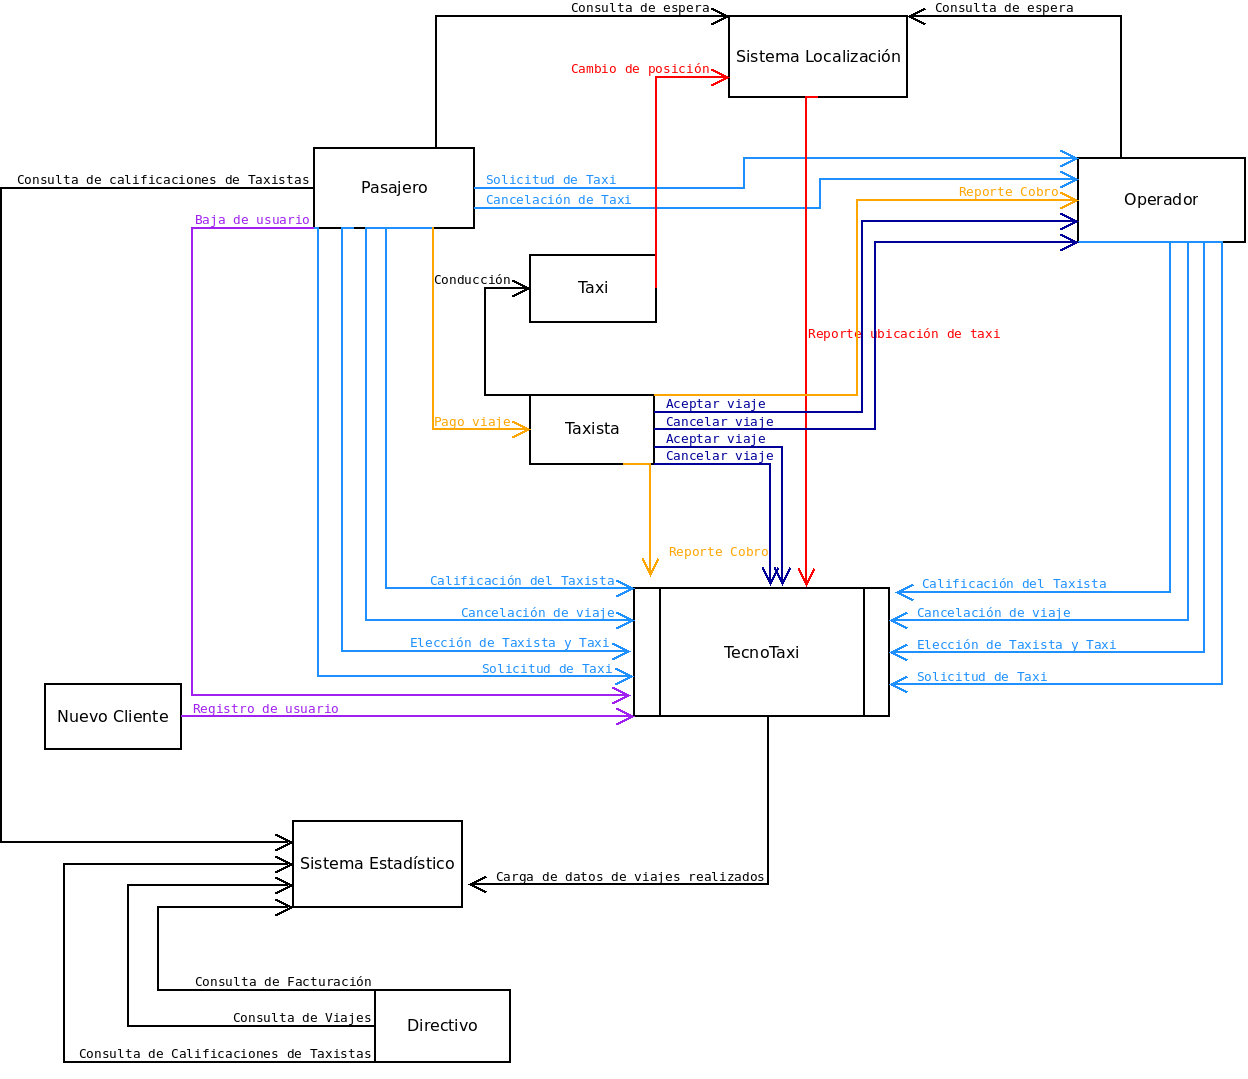
\includegraphics[scale=0.40]{diagramas/contexto/contextoAmpliado.png}
  \caption{Diagrama de contexto 1}
\end{figure}

\begin{figure}[h!]
  \centering    
    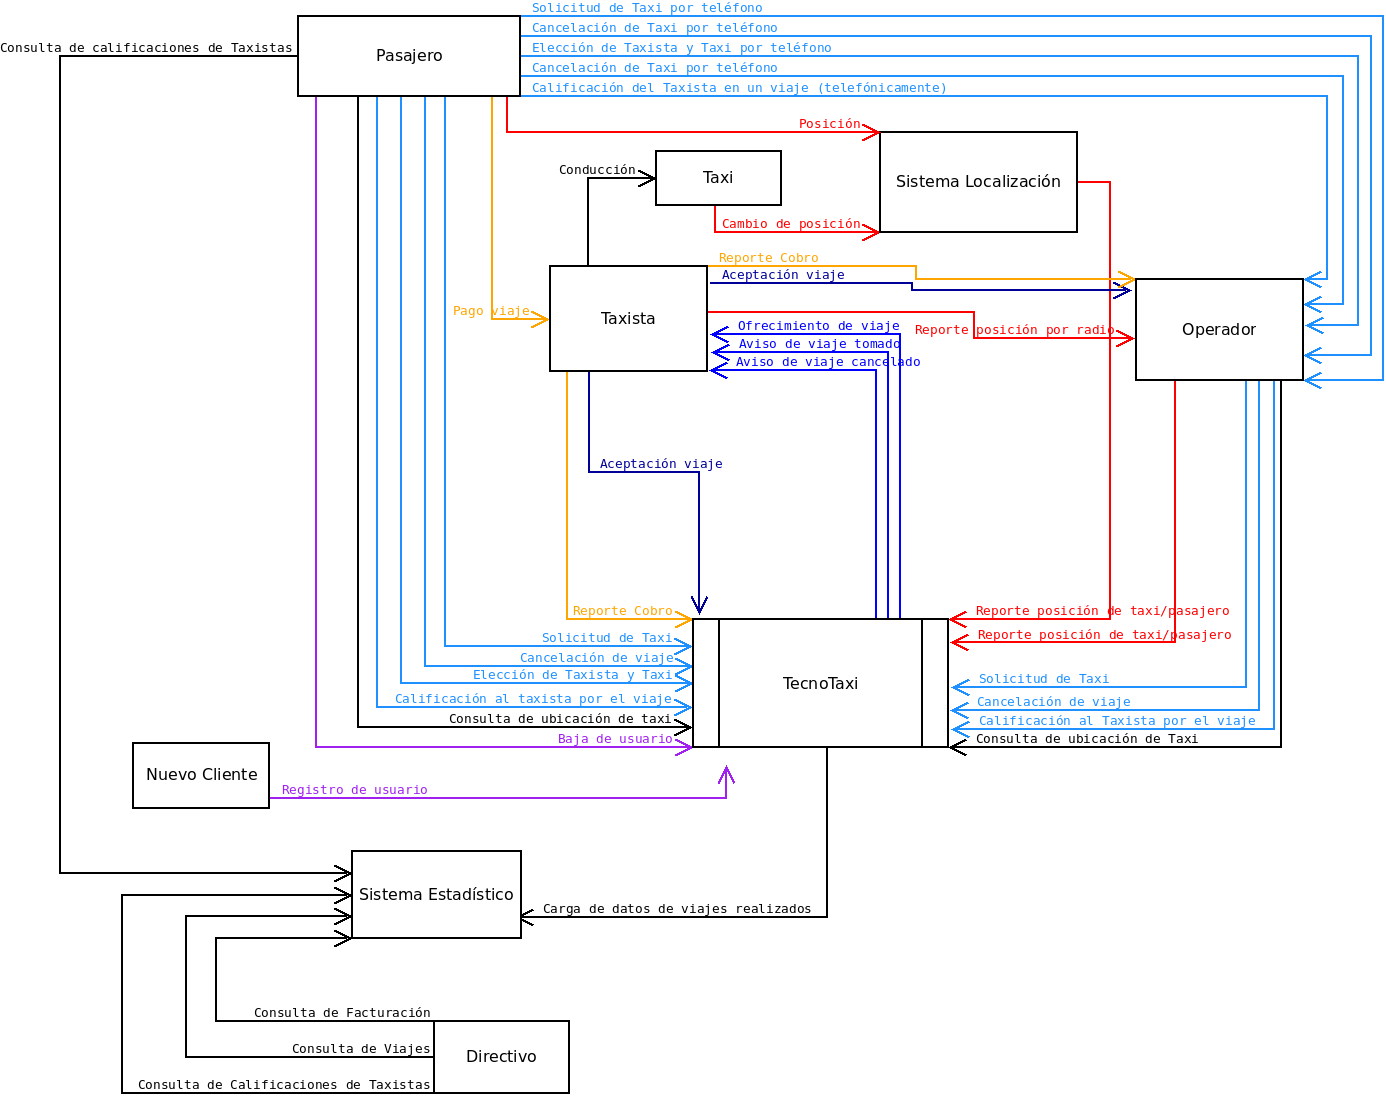
\includegraphics[scale=0.33]{diagramas/contexto/contextoAmpliado2.png}
  \caption{Diagrama de contexto 2}
\end{figure}

\begin{figure}[h!]
  \centering    
    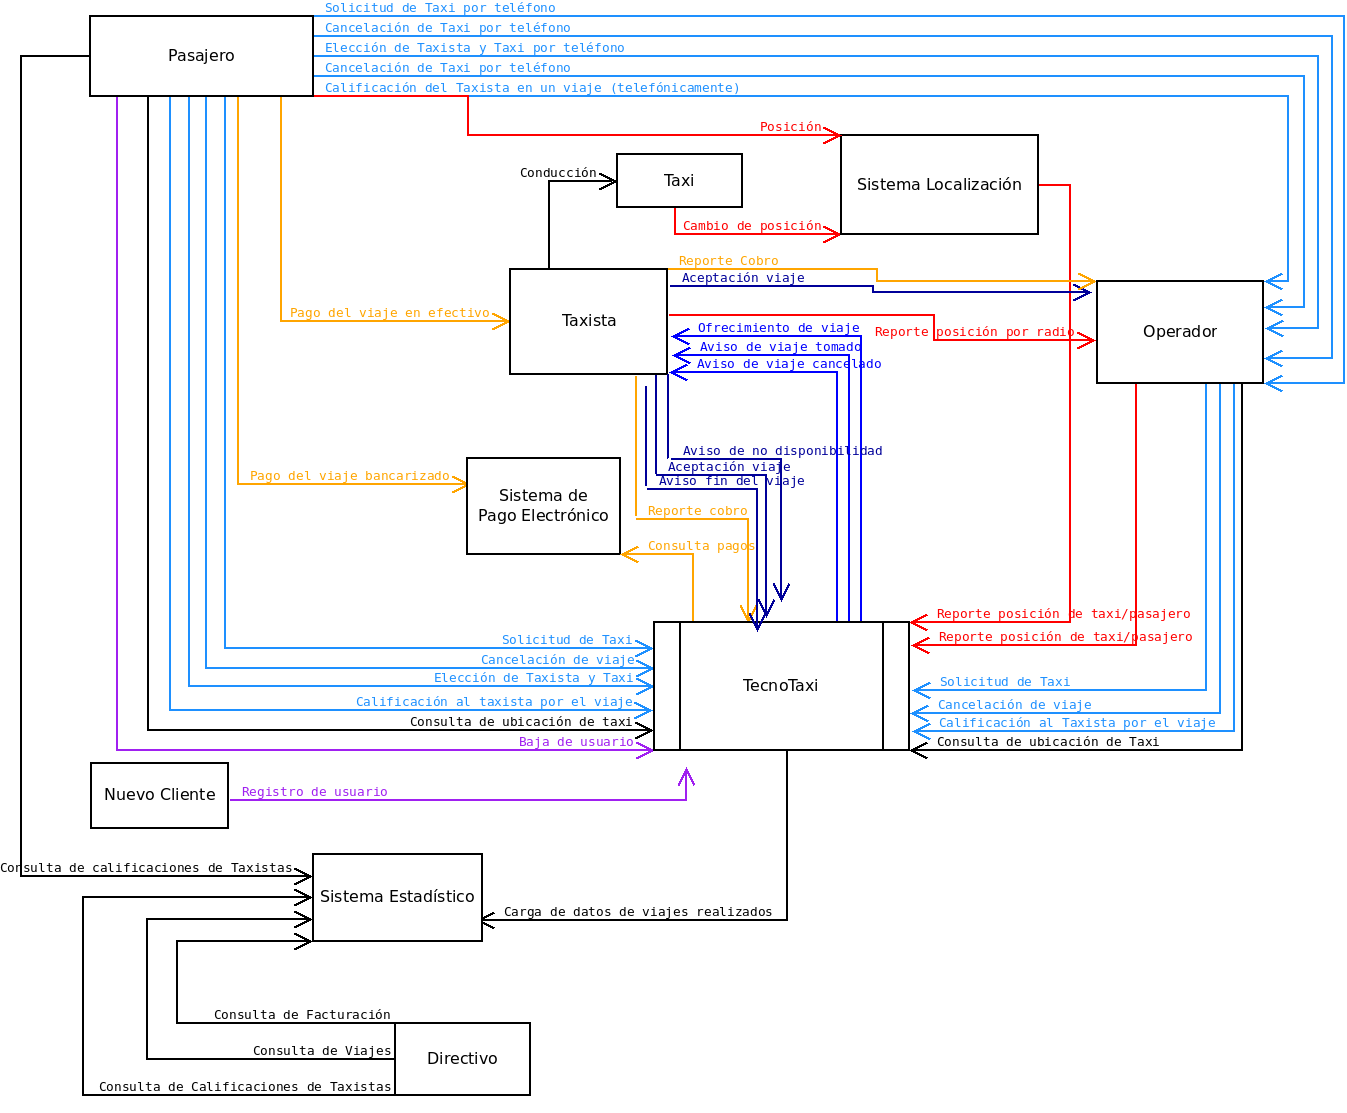
\includegraphics[scale=0.33]{diagramas/contexto/contextoAmpliado3.png}
  \caption{Diagrama de contexto 3}
\end{figure}

\subsection{Diagrama de objetivos}
Este diagrama fue partido en varios para mejorar la legibilidad dada la dimension. El primer diagrama muestra la raiz del arbol de objetivos con los hijos del primer nivel(desde arriba hacia abajo) y luego se muestran las imagenes de cada rama de ese primer nivel por separado.

\begin{figure}[h!]
  \centering        
    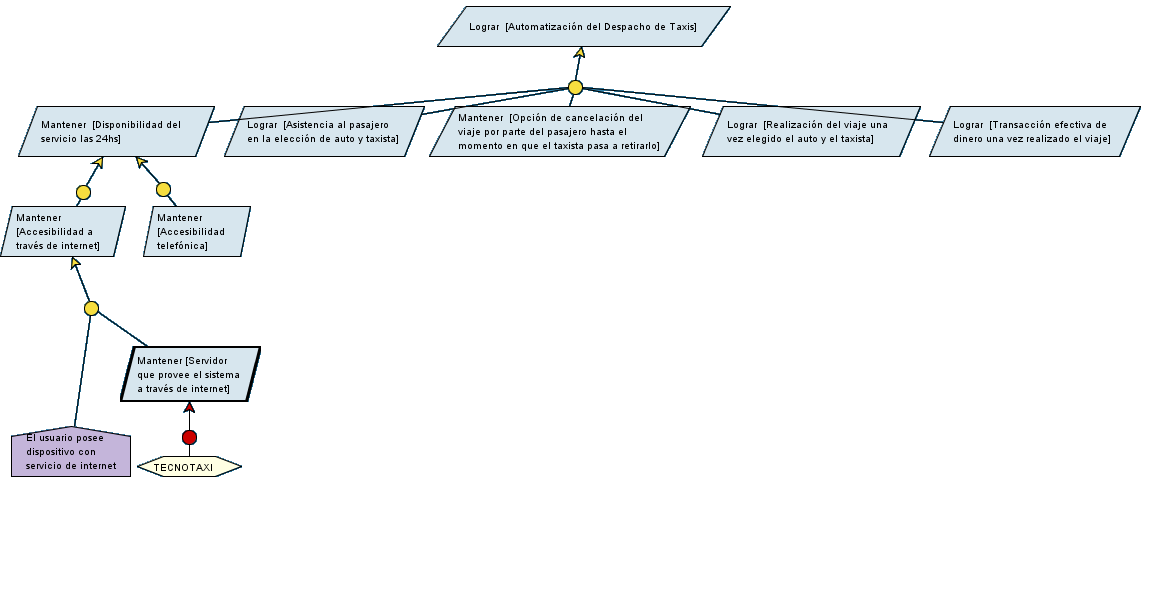
\includegraphics[scale=0.60]{diagramas/objetivos/objetivosrama1-main.png}
  \caption{Diagrama de objetivos: Raiz del arbol, rama 1 y ramas primer nivel\textbf{(los hijos de las ramas estan en las siguientes figuras)}}
\end{figure}

\begin{figure}[h!]
  \centering        
    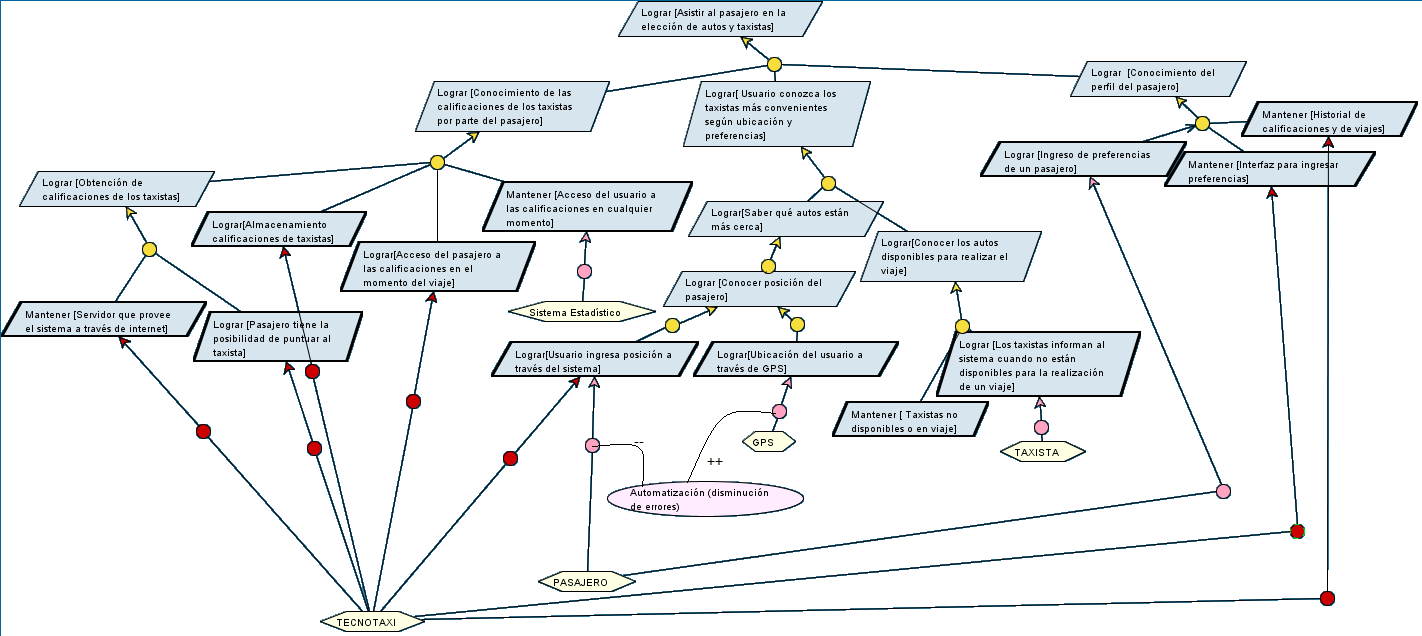
\includegraphics[scale=0.45]{diagramas/objetivos/objetivosrama2.png}
  \caption{Diagrama de objetivos: Rama 2}
\end{figure}

\begin{figure}[h!]
  \centering        
    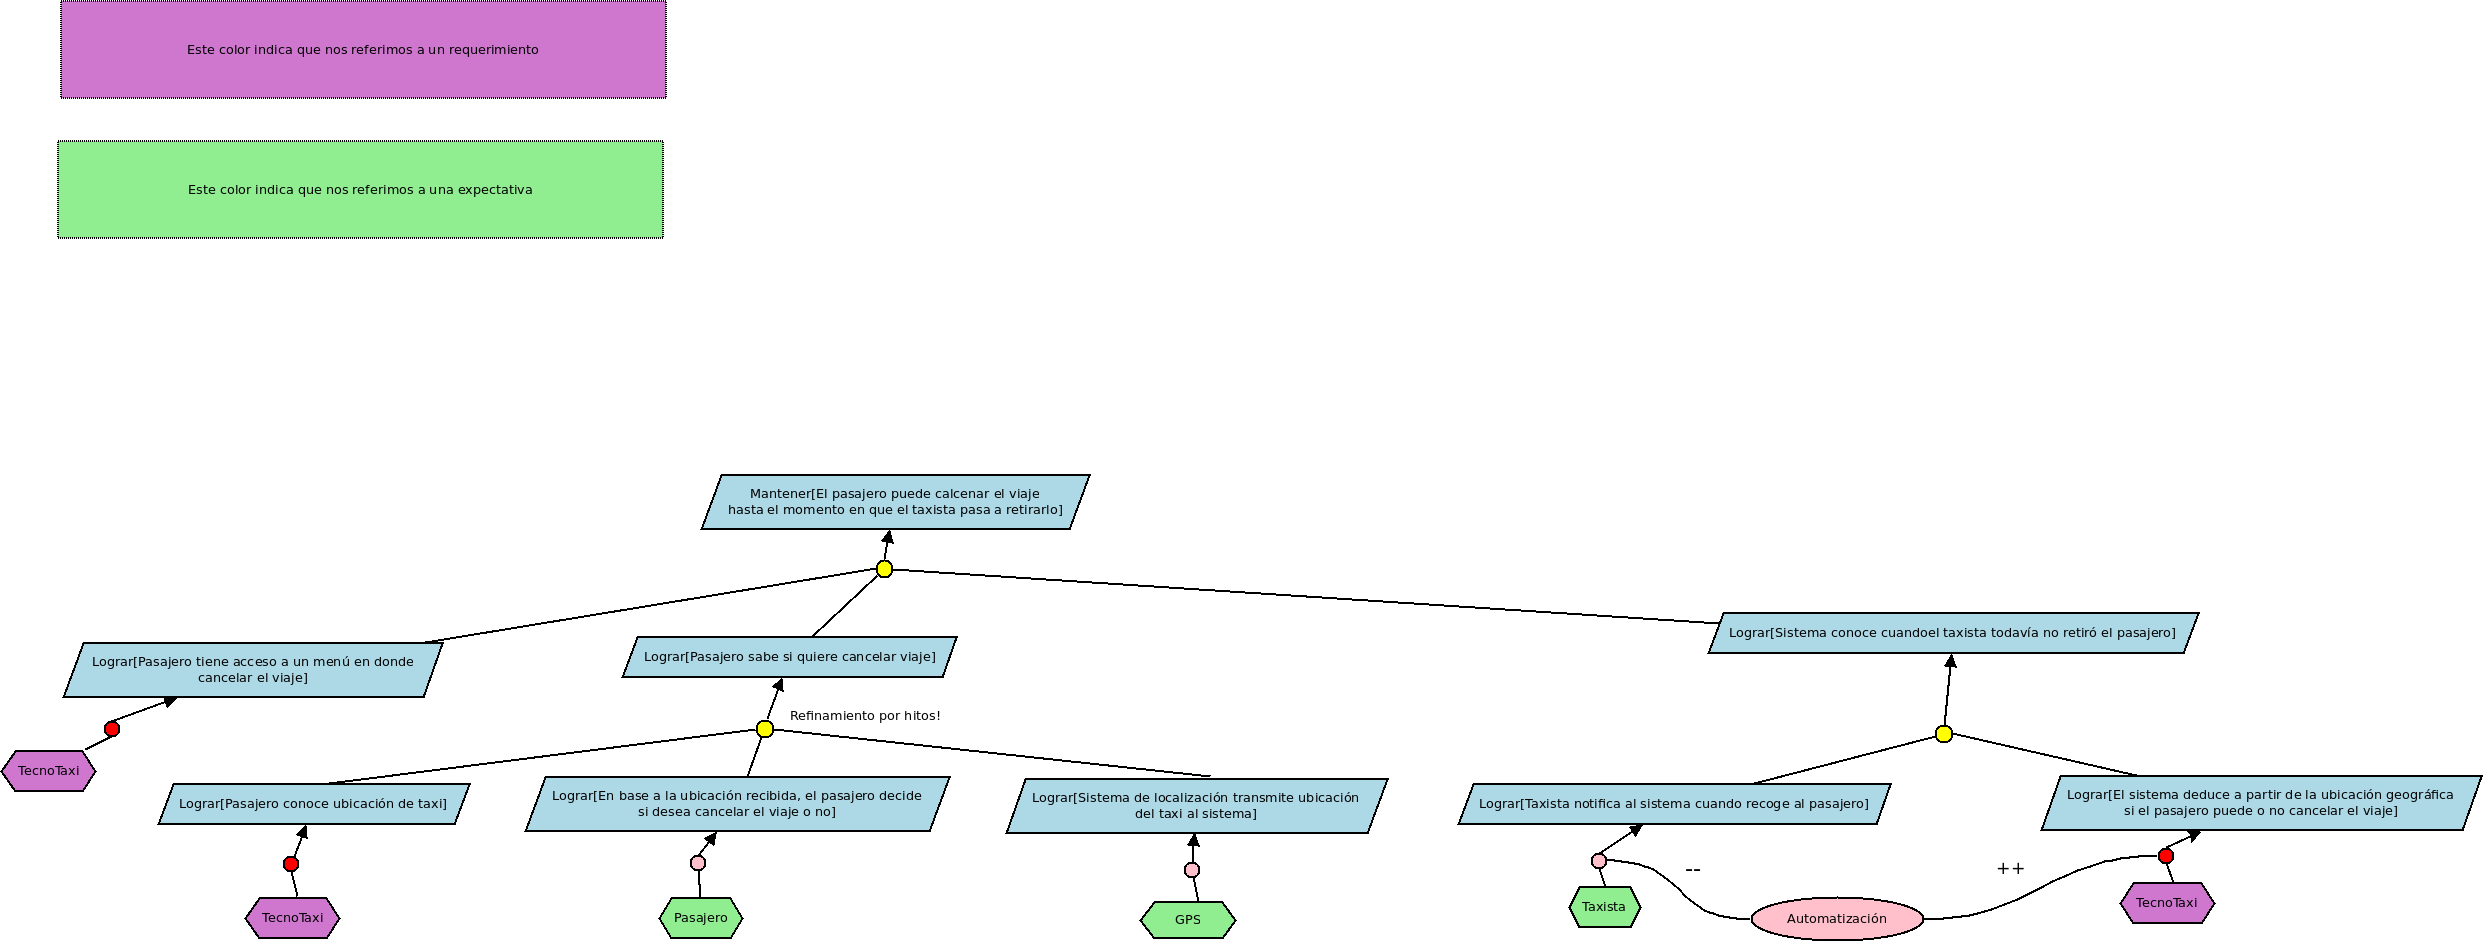
\includegraphics[scale=0.20]{diagramas/objetivos/objetivosrama3.png}
  \caption{Diagrama de objetivos: Rama 3}
\end{figure}

\begin{figure}[h!]
  \centering        
    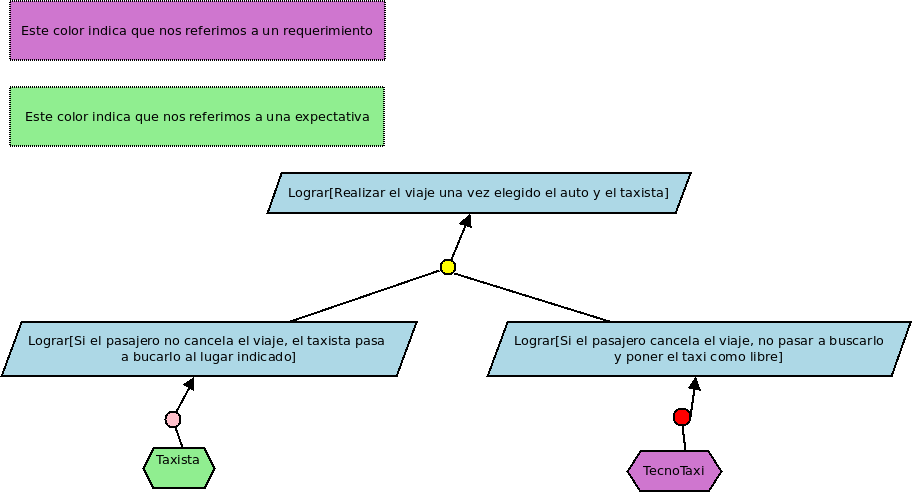
\includegraphics[scale=0.50]{diagramas/objetivos/objetivosrama4.png}
  \caption{Diagrama de objetivos: Rama 4}
\end{figure}

\begin{landscape}
\begin{figure}[h!]
  \centering        
    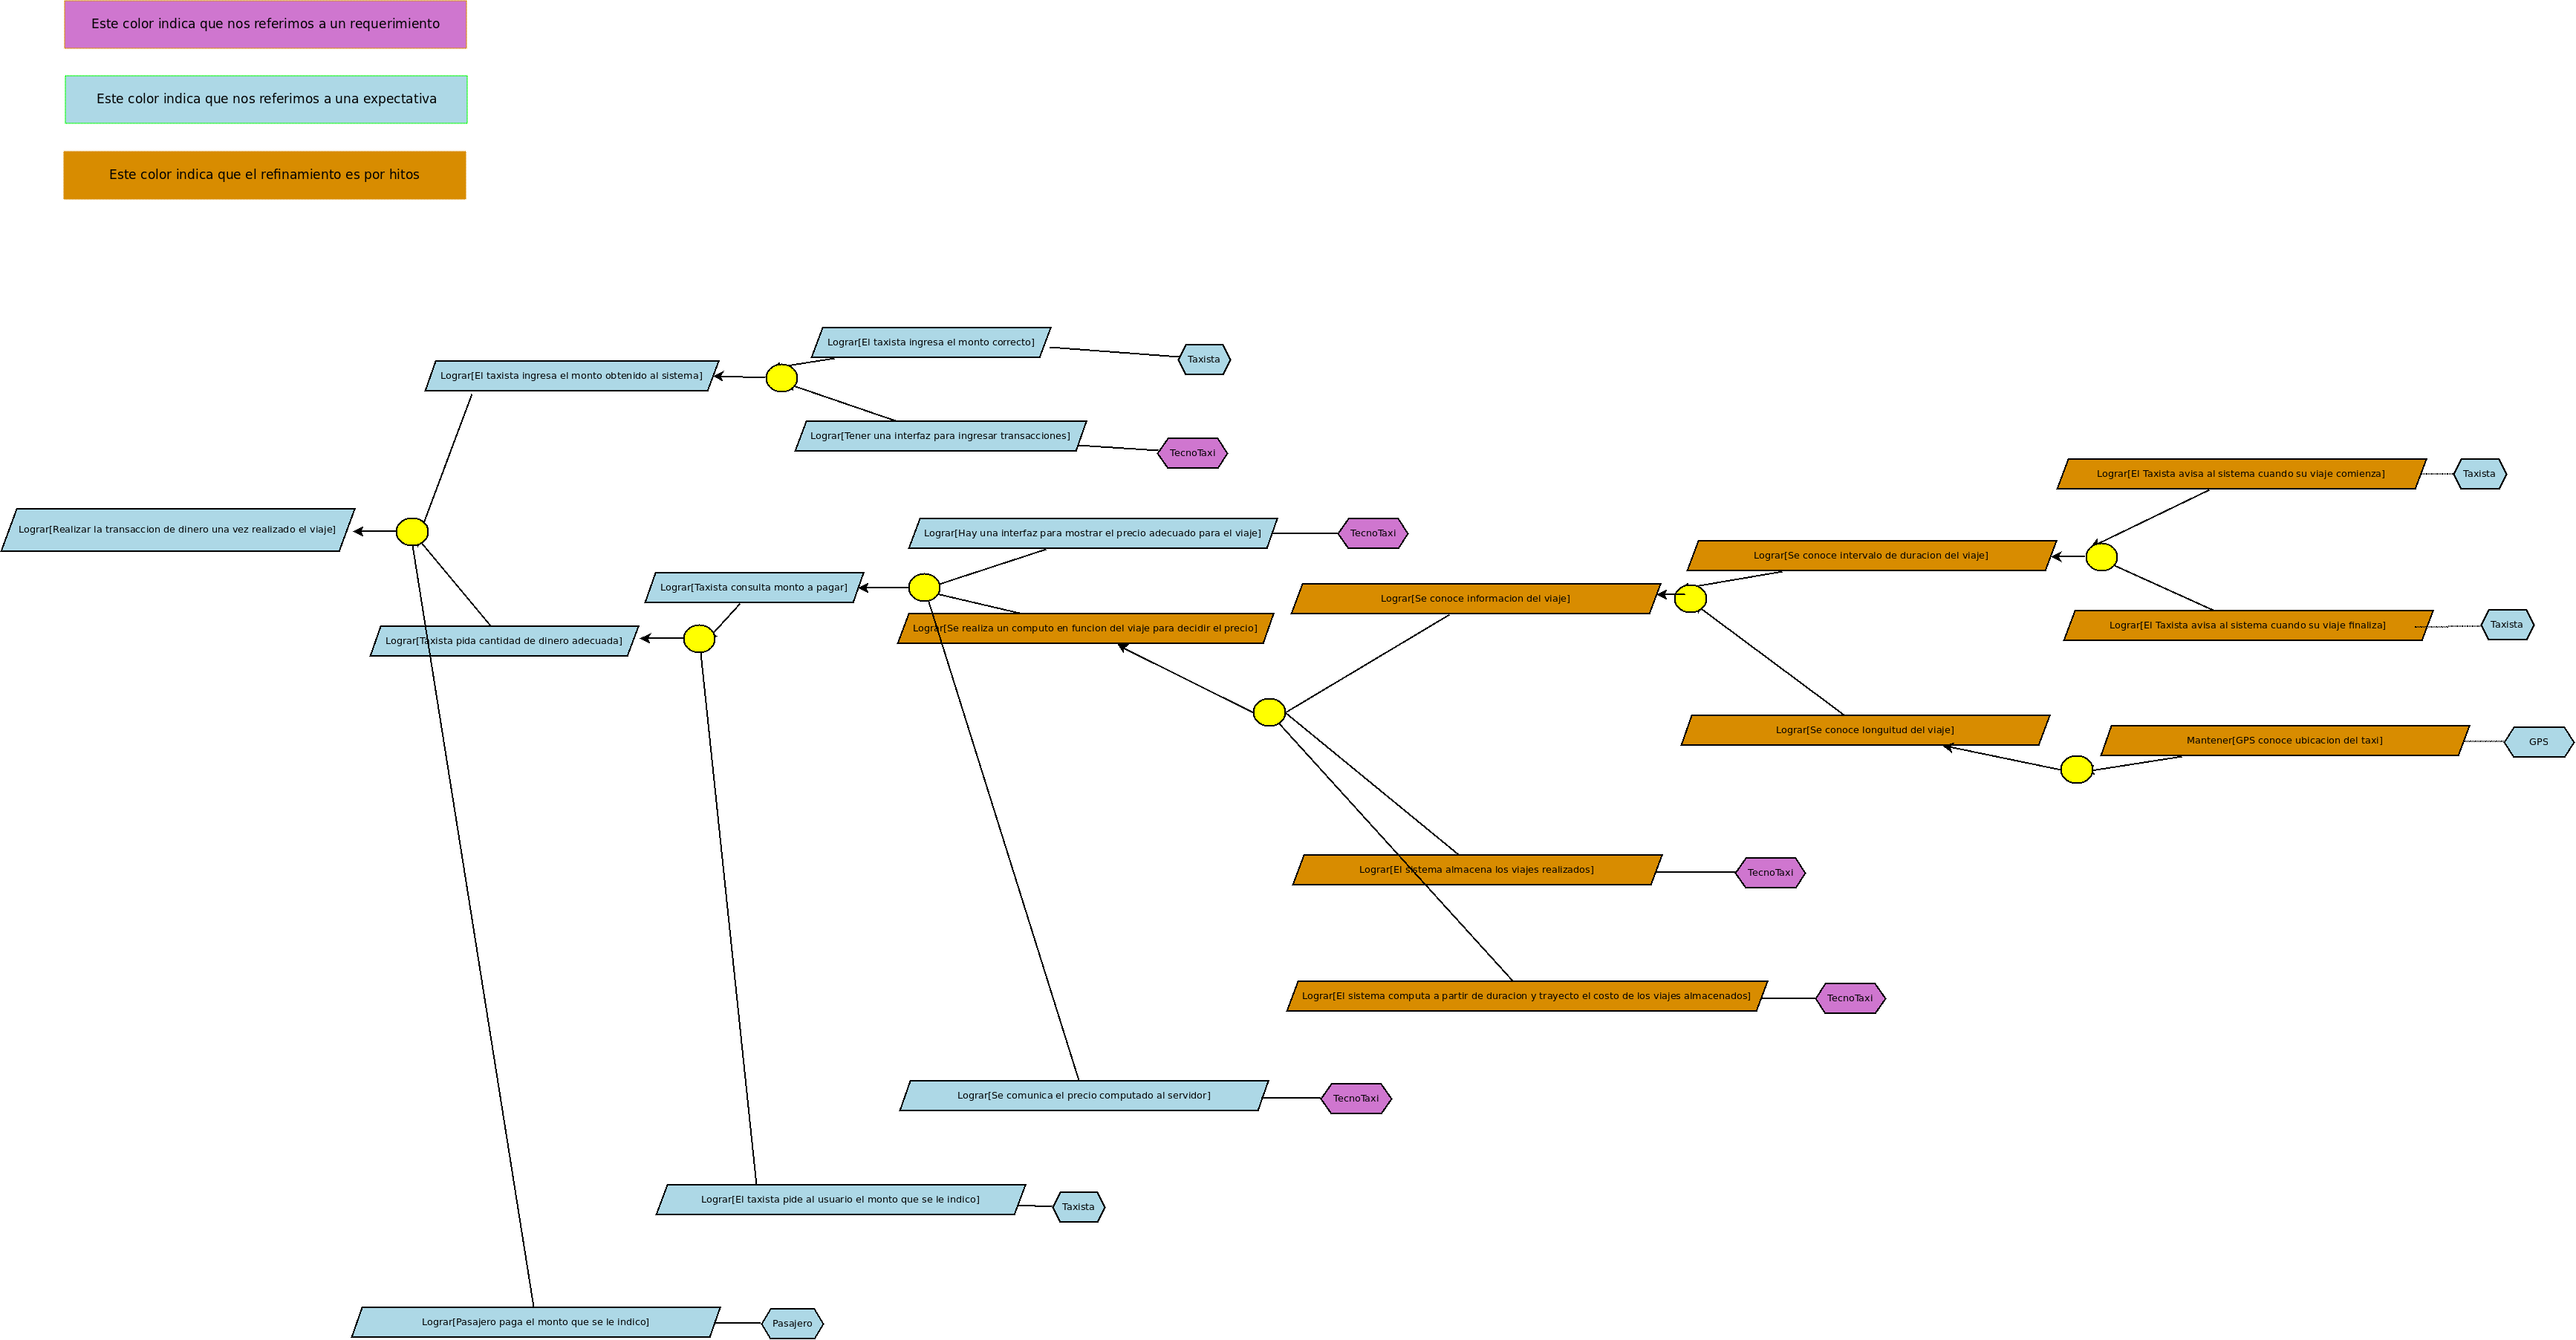
\includegraphics[scale=0.215]{diagramas/objetivos/objetivosrama5.png}
  \caption{Diagrama de objetivos: Rama 5}
\end{figure}
\end{landscape}

\subsubsection{Rama extra: Diagrama de objetivos: Estadisticas y directivos}
\begin{lstlisting}
*)Lograr[Directivos pueden consultar estadisticas del sistema]
    Mantener[Estadisticas del sistema]
        Mantener[Informacion de cada viaje] (TecnoTaxi)
        Mantener[Informacion de cada transaccion] (TecnoTaxi)
        Mantener[Informacion sobre los taxistas] (TecnoTaxi)
        Mantener[Informacion sobre los pasajeros] (TecnoTaxi)
    Lograr[Consultar informacion al sistema] Directivo (Directivo)

    Lograr[Mostrar la informacion mantenida en forma entendible]
    (refinamiento por casos)
        Lograr[Saber si la persona que pide informacion es un Directivo] (TecnoTaxi) ++Seguridad -- sistema sencillo
        Lograr[Si la persona es un Directivo mostrar la informacion de forma entendible] (TecnoTaxi)
        Lograr[Si la persona no es un Directivo no mostrar informacion] (TecnoTaxi)
            O-ref
        Lograr[Mostrar informacion pedida de forma entendible] ++ sistema sencillo --seguridad

\end{lstlisting}

\section{Casos de ejemplo}
\subsection{Caso: Viaje exitoso}
El pasajero desea viajar del punto A al punto B en auto. Para ello quiere contratar los servicios de TecnoTaxi, el primer paso que realiza es ingresar a su perfil via internet(o comunicarse con la operadora en caso de no estar familiarizado con la tecnologia) y solicitar un movil al sistema(o por medio de la operadora de ser necesario). El sistema computa una lista de taxistas disponibles y con caracteristicas deseadas por el pasajero, y se las presenta al pasajero, al este elegir un taxista, el sistema le comunica al taxista el nuevo viaje, en caso de que el taxista acepte, el pasajero es notificado que el movil esta en camino. El usuario puede verificar en el sistema(por medio de operadora o el sistema) el tiempo estimado de espera o cancelar el viaje. Cuando el taxista arriba y se realiza el viaje desde A hasta B, el taxista pide la cantidad adecuada de dinero y el pasajero entrega dicha cantidad(ver diagrama de objetivos para esta operacion). Al finalizar, el pasajero otorga una puntuacion al taxista y finaliza el servicio contratado por TecnoTaxi para este viaje.

\subsection{Caso: Sin internet}
1) Un usuario desea pedir un taxi para realizar un viaje, pero no posee ningún dispositivo con acceso a internet. Este se comunica telefónicamente con la operadora de RadioTaxi indicandole origen, destino y horario en el que desea el taxi. La operadora posee acceso directo a través de una red local al sistema, a través de una interfaz reducida carga manualmente los datos para el viaje y el sistema se encarga de asignarle el viaje a un taxista notificando al mismo. Una vez asignado el viaje, se comunica a la operadora el taxista encargado y esta a su vez comunica al cliente. En caso de no poseer ningún taxi disponible el sistema lo indicará y la operadora informará al cliente de la misma manera. Una vez que el taxista retire al pasajero, el resto del viaje continua con su curso normal.

\subsection{Caso: Caida de conexion a internet y solucion de contingencia}
2) Durante un viaje el taxista deja de tener acceso a internet. La interfaz que este posee dentro de su veh\'iculo lo notifica y la comunicación durante este per\'iodo será exclusivamente a través de la radio con la operadora, indicando cuando concrete sus viajes y siendo notificado cuando le es asignado un viaje. La operadora se encargará de mantener la consistencia en el sistema cargando manualmente lo que cargar\'ia durante el transcurso de un viaje normal el taxista, es decir la finalización de los viajes, las transacciones de dinero, la cancelación de un viaje por no disponibilidad, etc.

\end{document}